
{\sl This fieldstone was developed in collaboration with Lukas van de Wiel}.

The domain is an annulus with inner radius $R_1$ and outer radius $R_2$. It is filled with a 
single elastic material characterised by a Young's modulus $E$ and a Poisson ratio $\nu$, a
density $\rho_0$. The gravity ${\bm g}=-g_0 {\bm e}_r$ is pointing towards the center of the domain.

{\color{red} $2\mu$ is missing!}

Given these assumptions, the momentum Stokes equations in the annulus are~\cite{scto01}
\begin{eqnarray}
   \frac{\partial^2 v_r}{\partial r^2} + \frac{1}{r} \frac{\partial v_r}{\partial r} +   
      \frac{1}{r^2} \frac{\partial^2 v_r}{\partial \theta^2}
    - \frac{v_r}{r^2} - \frac{2}{r^2} \frac{\partial u_\theta}{\partial \theta} 
-\frac{\partial p}{\partial r}  &=& \rho g_r \label{eq1} \\
\frac{\partial^2 v_\theta}{\partial r^2} + \frac{1}{r} \frac{\partial v_\theta}{\partial r} + \frac{1}{r^2} \frac{\partial^2 v_\theta}{\partial \theta^2}
+\frac{2}{r^2} \frac{\partial v_r}{\partial \theta} - \frac{v_\theta}{r^2} 
-\frac{1}{r}\frac{\partial p}{\partial \theta} &=& 0
\label{eq2} 
\end{eqnarray}
Equations (\ref{eq1}) and (\ref{eq2}) are the momentum equations in polar coordinates.
The problem at hand is axisymmetric so that the tangential component of the displacement
vector $v_\theta$ is assumed to be zero as well as all terms containing $\partial_\theta$.
Under these assumptions the second equation is automatically fulfilled.
Of the first one remain the following terms:
\[
\frac{\partial^2 v_r}{\partial r^2} + \frac{1}{r} \frac{\partial v_r}{\partial r} - \frac{v_r}{r^2} 
-\frac{\partial p}{\partial r}  = \rho g_r 
\]
As we have seen before we have 
\[
p=-\lambda {\bm \nabla}\cdot {\bm v}
= -\lambda \left( \frac{1}{r} \frac{\partial (r v_r)}{\partial r} \right)
\]
Inserting this expression into the first equation yields:
\[
\frac{\partial^2 v_r}{\partial r^2} + \frac{1}{r} \frac{\partial v_r}{\partial r} - \frac{v_r}{r^2} 
= \frac{\rho g_0 }{2\mu + \lambda}
\]
We now look at the boundary conditions. On the inner boundary we prescribe $v_r(r=R_1)=0$ while free
surface boundary conditions are prescribed on the outer boundary, i.e. ${\bm \sigma}\cdot{\bm n}=0$
(i.e. there is no force applied on the surface).

The components of the strain tensor are 
\begin{eqnarray}
\varepsilon_{rr} &=& \frac{\partial v_r}{\partial r} \\
\varepsilon_{\theta\theta} &=& \frac{v_r}{r} + \frac{1}{r} \frac{\partial v_\theta}{\partial \theta}
= \frac{v_r}{r} 
 \\
\varepsilon_{r\theta} &=& \frac{1}{2} \left(   \frac{\partial v_\theta}{\partial r} - \frac{v_\theta}{r} 
+\frac{1}{r} \frac{\partial v_r}{\partial \theta}  \right) =0
\end{eqnarray}
The stress tensor is given by 
\[
{\bm \sigma} 
= - p {\bm 1} + 2\mu {\bm \varepsilon}
=  \lambda ({\bm \nabla}\cdot {\bm v}) {\bm 1} + 2\mu {\bm \varepsilon}
\]
which is a diagonal tensor so that the free surface condition is:
\[
\sigma_{rr} = (2\mu+\lambda) \frac{\partial v_r}{\partial r} +\lambda \frac{v_r}{r}   =0 \quad\quad r=R_2
\]
The solution is then 
\[
v_r(r) =  \frac{\rho g_0 }{3(2\mu + \lambda)} r^2 + br + \frac{c}{r}
\]
where $b,c$ are determined by means of the boundary conditions.


\begin{center}
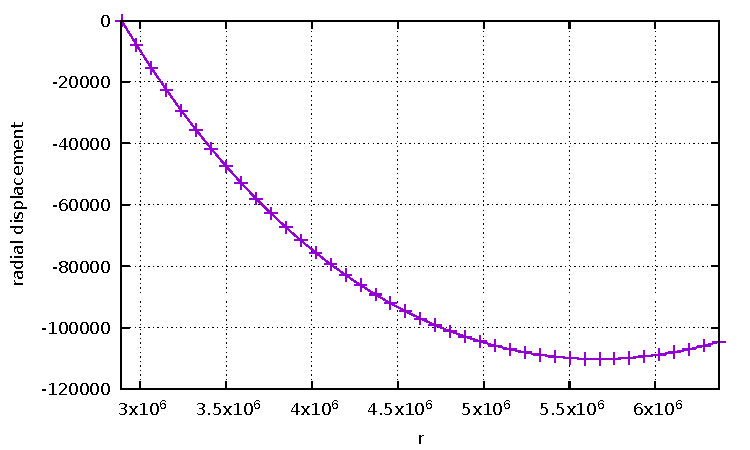
\includegraphics[width=7cm]{python_codes/fieldstone_36/displacement_rtheta.pdf}
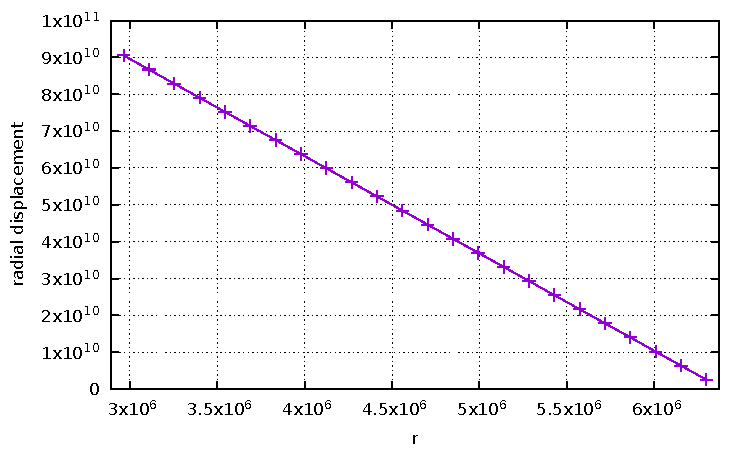
\includegraphics[width=7cm]{python_codes/fieldstone_36/pressure_rtheta.pdf}
\end{center}

\begin{center}
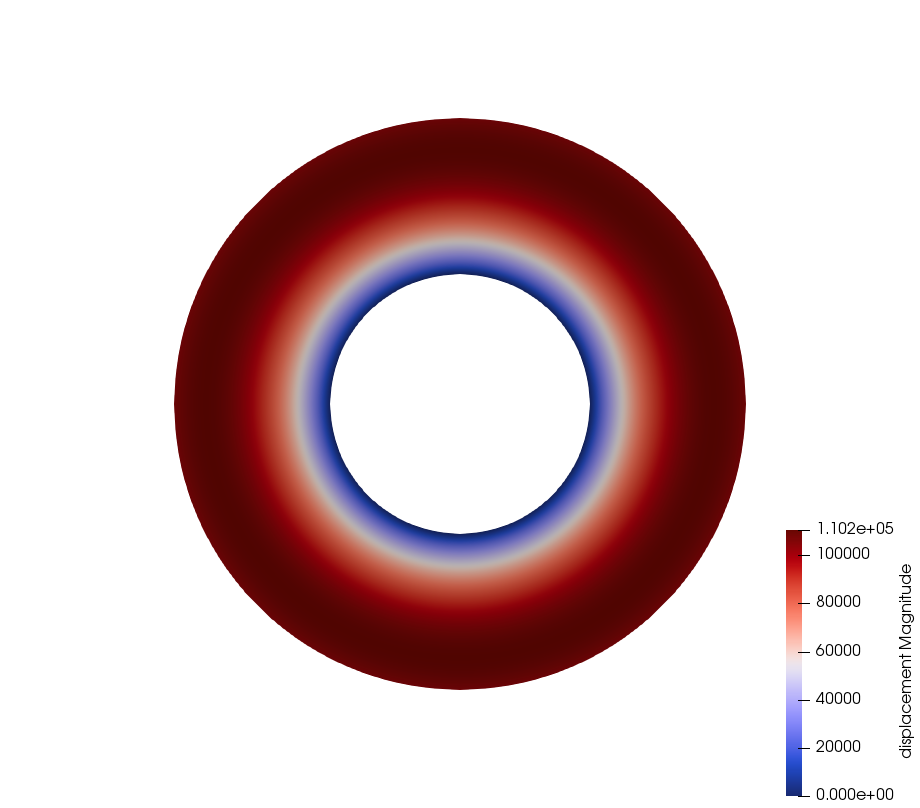
\includegraphics[width=6cm]{python_codes/fieldstone_36/disp}
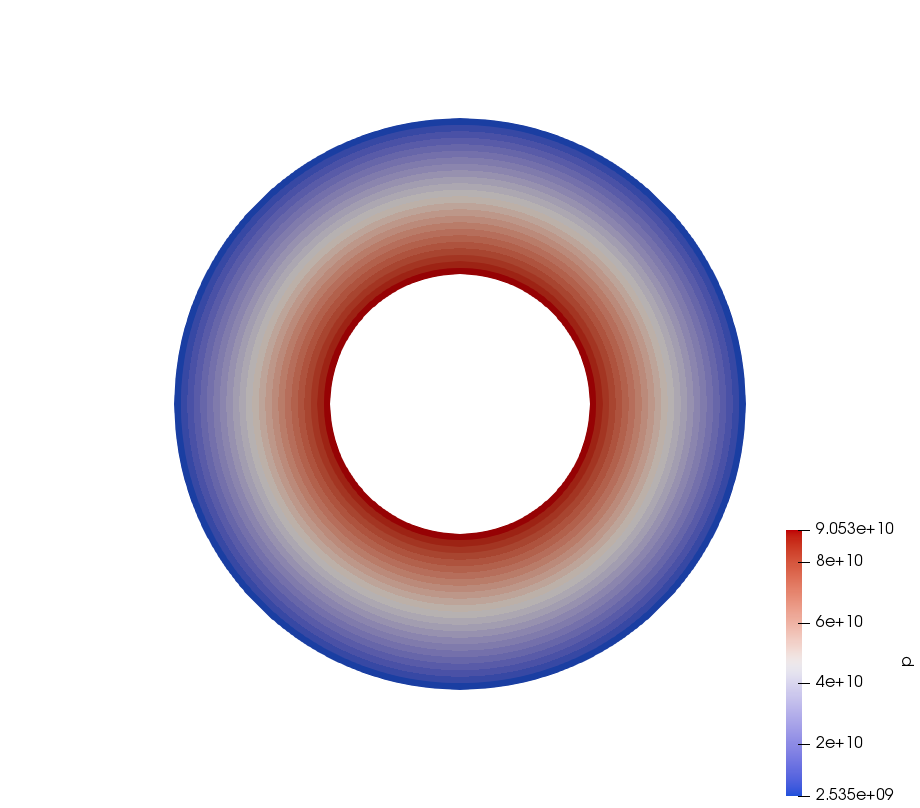
\includegraphics[width=6cm]{python_codes/fieldstone_36/p}
\end{center}

code not finished

do resolution error rates


